\documentclass[10pt]{beamer}
%\usetheme{Boadilla}
%\usecolortheme{beaver}
%\usepackage[latin1]{inputenc}
\useoutertheme{split}
\setbeamertemplate{navigation symbols}{}
\usefonttheme[onlymath]{serif}
\usepackage{amsmath}%
\usepackage{amsthm}%
\usepackage{amsfonts}%
\usepackage{amssymb}%
\usepackage[algo2e]{algorithm2e}
\usepackage{algorithmic}  
\usepackage{algorithm}
\usepackage{tikz}
\usepackage[english]{babel}
\usepackage{amsmath, amssymb, amsthm}
\usepackage{verbatim}
\usepackage{mathrsfs}
%\usepackage{epstopdf}
\usepackage{graphicx}
\mode<presentation>
{
	\usetheme{CambridgeUS}
	\usecolortheme{dolphin}
	\usecolortheme{rose}
	\setbeamercovered{transparent}
}
\newcommand{\mrel}{\mathrel{\bigcirc}}
%\usepackage[onehalfspacing]{setspace}
%\setbeamertemplate{footline}[frame number]
\DeclareMathOperator*{\Bigcdot}{\scalerel*{\cdot}{\bigodot}}
% Macros
\def\a{\alpha} \def\b{\beta} \def\c{\gamma} \def\d{\delta} \def\r{\rho}
\def\e{\epsilon} \def\ve{\varebsilon} \def\k{\kappa} \def\p{\pi} \def\th{\theta}
\def\l{\lambda} \def\m{\mu} \def\s{\sigma} \def\t{\tau} \def\w{\omega} \def\z{\zeta}
\def\D{\Delta} \def\G{\Gamma} \def\W{\Omega} \def\P{\Phi} \def\L{\Lambda}
\def\bdm{\begin{displaymath}} \def\edm{\end{displaymath}}
\def\bni{\begin{itemize}} \def\ei{\end{itemize}}
\def\bnen{\begin{enumerate}} \def\een{\end{enumerate}}
\def\fa{\forall}
\def\be{\begin{equation}} \def\ee{\end{equation}}
\def\fn{\footnote} \def\bn{\begin} \def\nit{\noindent}
\def\iff{\textit{~if and only if~~}}
\renewcommand*{\thefootnote}{\fnsymbol{footnote}}
% THEOREMS -------------------------------------------------------
\newtheorem{thm}{Theorem}%[section]
\newtheorem{cor}[thm]{Corollary}
\newtheorem{lem}[thm]{Lemma}
\newtheorem{prop}[thm]{Proposition}
\newtheorem{claim}{Claim}
\theoremstyle{definition}
%\newtheorem{defn}[thm]{Definition}
\theoremstyle{remark}
\newtheorem{rem}[thm]{Remark}
%%\numberwithin{equation}{section}  
 
\newcommand{\N}{\mathbb{N}}
\newcommand{\Z}{\mathbb{Z}}
\newcommand{\R}{\mathbb{R}}
\newcommand{\ls}{\left\{}
\newcommand{\rs}{\right\}}


\title[Interaction-Partitioned Topic Model (IPTM)]{ \vspace{-.25cm} \\ A Network Model for \\Dynamic Textual Communications \\with Application to
	Government Email Corpora}
\author[\quad B. Kim, A. Schein, B. Desmarais and H. Wallach\quad]{
Bomin Kim\textsuperscript{1}\and
\quad Aaron Schein\textsuperscript{3}\and\\
		Bruce Desmarais \textsuperscript{1}\and Hanna Wallach\textsuperscript{2,3}}
\institute{\textsuperscript{1} The Pennsylvania State University \and \textsuperscript{2} Microsoft Research NYC \and \textsuperscript{3} University of Massachusetts Amherst}


\begin{document}
 
\begin{frame}
  \titlepage
  \begin{center}
   \begin{tabular}{cc}
\hspace*{-.2in} \tiny \begin{minipage}{3.5in}
Work supported by NSF grants SES-1558661, SES-1619644, SES-1637089, and CISE-1320219)\\ ~\\~\\~\\~\\
\end{minipage}
& \includegraphics[scale=.05]{figures/NSF_logo.png}
\end{tabular}
\end{center}
\end{frame}


\begin{frame}{Interaction-Partitioned Topic Model (IPTM)}
	\bni
	\item Probablistic model for time-stamped textual communications \\
	\vspace{0.2cm}
	\item Integration of two generative models:\\
		\vspace{0.1cm}
	 - Latent Dirichlet allocation (LDA) for topic-based contents\\	\vspace{0.2cm}
	 - Dynamic exponential random graph model (ERGM) for ties \\
	\ei
		\vspace{0.4cm}
\centering \large\textit{``who communicates with whom about what, and when?"}
\end{frame}

\begin{frame}{Content Generating Process: LDA (Blei et al., 2003)}
\bni 
\begin{minipage}{0.7\linewidth}
\item For each topic $k =1,...,K:$\vspace{0.2cm}
	\begin{itemize}
		\item[1.] Choose a topic-word distribution over the word types\vspace{0.2cm}
		\item[2.] Choose a topic-interaction pattern assignment			
		\end{itemize}
		\vspace{0.2cm}
	\end{minipage}
	\begin{minipage}{0.25\linewidth}
			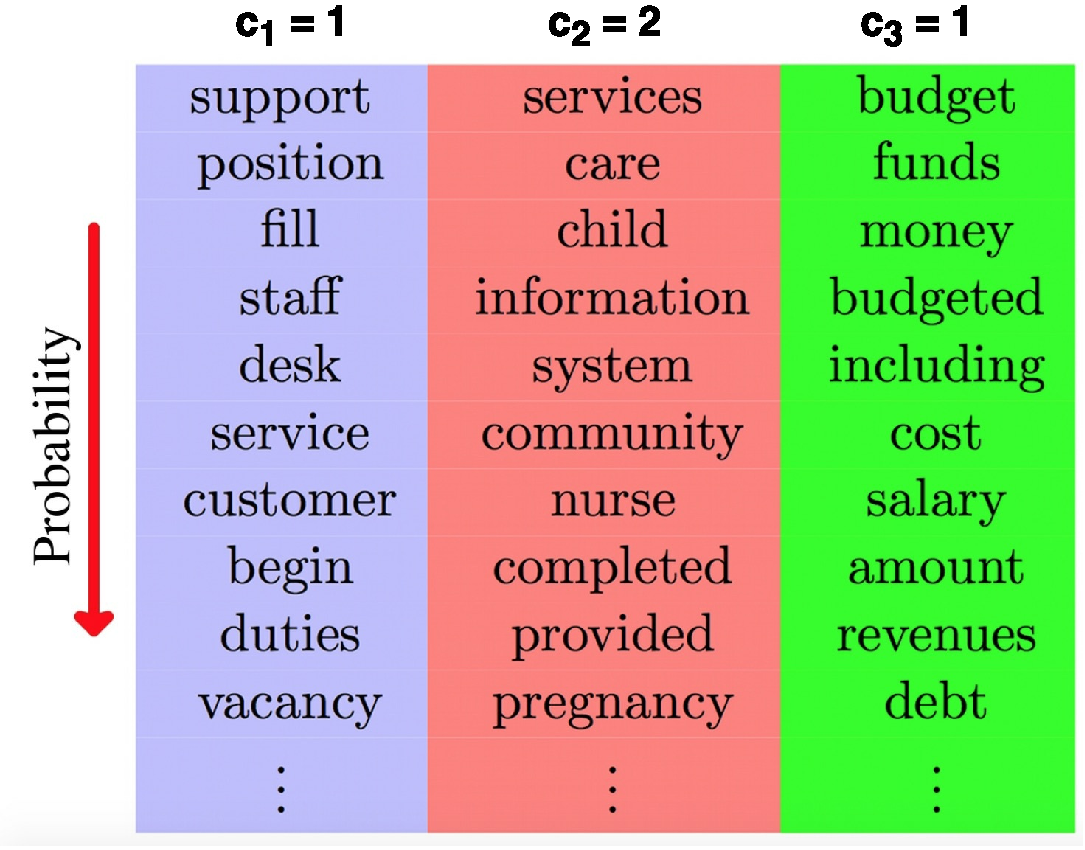
\includegraphics[width=1\textwidth]{figures/word.pdf}
				\vspace{0.2cm}
		\end{minipage}
			\begin{minipage}{0.68\linewidth}
				\item For each document $d =1,...,D:$ \vspace{0.2cm}
		\begin{itemize}
					\item[3-1.] Choose a document-topic distribution \\\vspace{0.1cm} 
		\item[3-2.] For each word in a document $n=1$ to $N^{(d)}$:\vspace{0.1cm} 
		\begin{itemize}
			\item[(a)] Choose a topic from document-topic distribution\vspace{0.2cm} 
			\item[(b)] Choose a word from topic-word distribution
		\end{itemize} 
			\end{itemize}
		\end{minipage}
		\begin{minipage}{0.3\linewidth}
	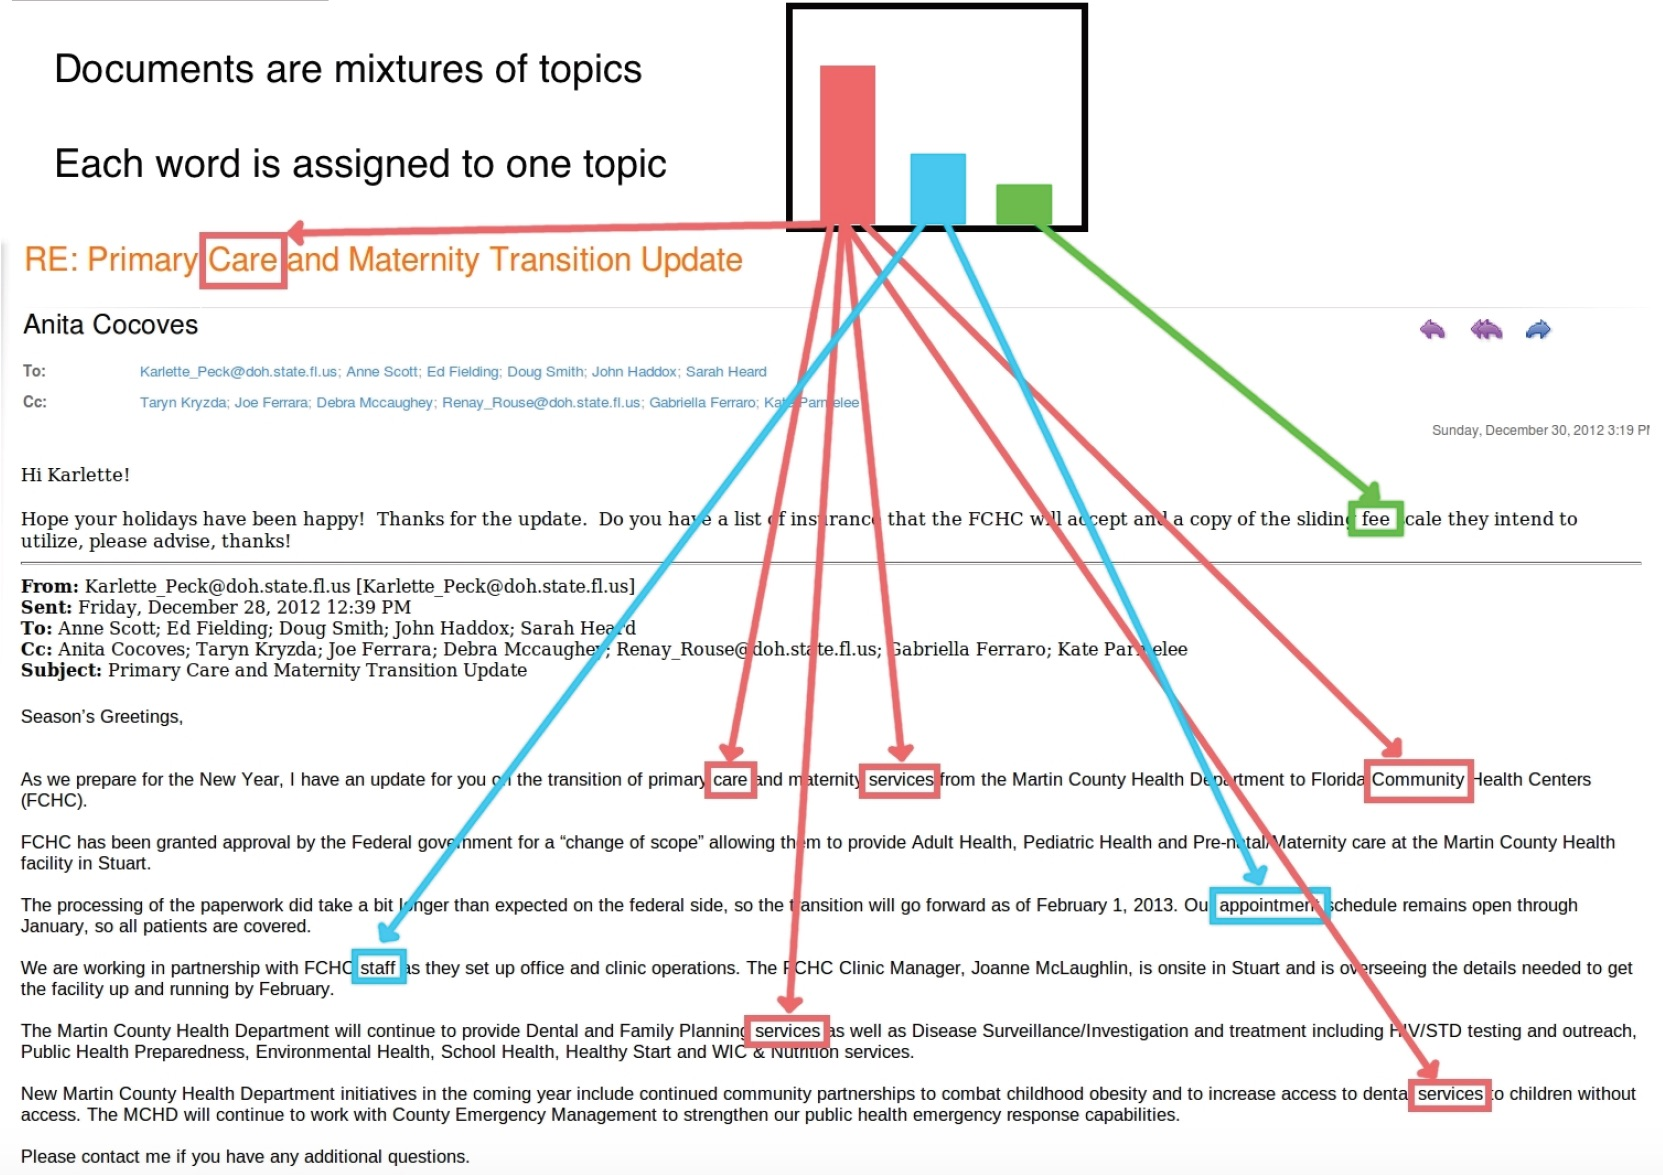
\includegraphics[width=1.05\textwidth]{figures/LDAimage.jpeg}
		\end{minipage}
		\vspace{0.2cm}
				\begin{itemize}\item[3-3] Calculate the distribution of interaction patterns within a document:
		 \footnotesize\begin{equation*}
		p_c^{(d)} = \Big({\sum\limits_{k: c_k=c} N^{(k|d)}}\Big)/{N^{(d)}},
		\end{equation*}\normalsize
	\end{itemize}
\ei	
\end{frame}


\begin{frame}{Dynamic Network Features (Perry and Wolfe, 2012)}
	\bni
	\item Partition the past 384 hours (=16 days) into 3 sub-intervals
	\footnotesize
	\begin{equation*}
	[t-384h,t) = [t-384h, t-96h) \cup [t-96h, t-24h)\cup [t-24h, t),
	\end{equation*}
	\normalsize
	then define the interval-based dynamic network statistics $(l = 1, 2, 3)$\\ \vspace{0.4cm}
	 \item $\boldsymbol{x}^{(c)}_{t, l}(i, j)$ is the network statistics at time $t$, for interaction pattern $c$ \\\vspace{0.1cm}
	- Degree: outdegree and  indegree\\\vspace{0.1cm}
 - Dyadic: send and receive \\\vspace{0.1cm}
 - Triadic: 2-send, 2-receive, sibling and cosibling\\\vspace{0.2cm}
	 \begin{figure}
	 	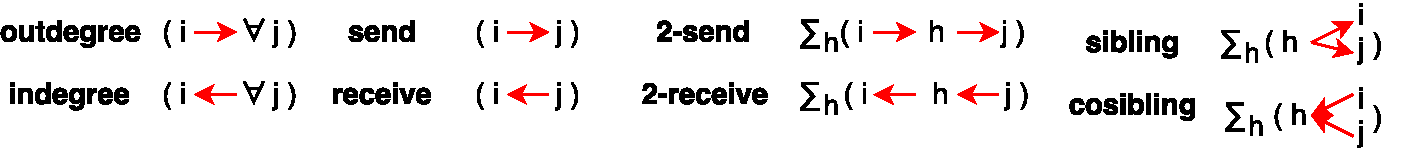
\includegraphics[width=0.9\textwidth]{figures/netstats.pdf}
	 \end{figure}	
	 \ei
\end{frame}

\begin{frame}{Tie Generating Process: Receivers}
		\begin{itemize}
		\item [1.] For each sender $i \in \{1,...,A\}$ and receiver $j \in \{1,...,A\}$, calculate the stochastic indensity between $i$ and $j$:
		\footnotesize
			\begin{equation*}\lambda^{(d)}_{ij}=\sum\limits_{c=1}^{C} p^{(d)}_c
		\cdot  \mbox{exp}\Big\{\boldsymbol{b}^{(c)}_0 + \boldsymbol{b}^{(c)T}\boldsymbol{x}^{(c)}_{t^{(d-1)}}(i, j)\Big\},	\end{equation*}\normalsize
		which is a mixture of contents, baseline interaction rate, and network effects.\\ \vspace{0.4cm}
		\item[2.] For each sender $i \in \{1,...,A\}$, choose a binary vector $J^{(d)}_i$ of length $(A-1)$, by applying Gibbs measure (Fellows and Handcock, 2017) 
		\footnotesize
		%\mbox{log}\big(\text{I}( \sum_{j \in \mathcal{A}_{\backslash i}} J^{(d)}_{ij} > 0 )\big) + 
		\begin{equation*} \text{P}(J_i^{(d)}) \propto \exp\Big\{ \sum_{j \in \mathcal{A}_{\backslash i}} (\delta+\mbox{log}(\lambda_{ij}^{(d)}))J_{ij}^{(d)} \Big\},
		\end{equation*}
		\normalsize
		where $\delta$ is a real-valued intercept controlling the recipient size\\ \vspace{0.1cm}
 \begin{figure}
 	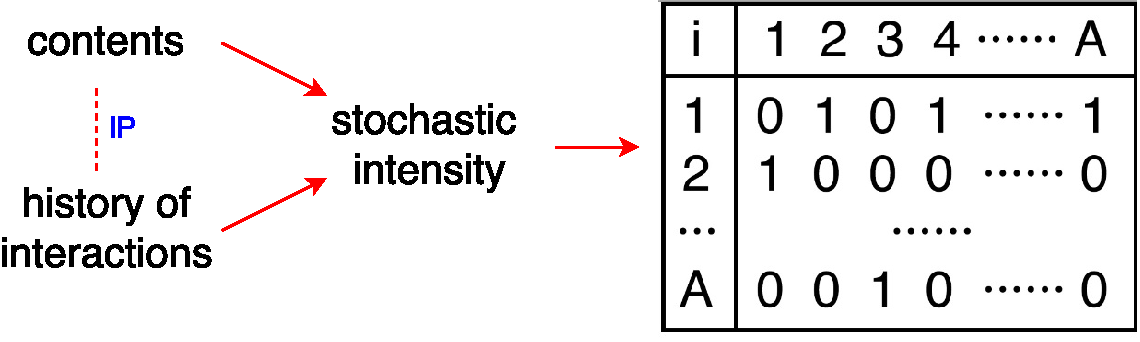
\includegraphics[width=0.5\textwidth]{figures/edge.pdf}
 \end{figure}	
	\end{itemize}
	\end{frame}
\begin{frame}{Tie Generating Process: Sender and Time}
\begin{itemize}
		\item [3.] For each sender $i \in \mathcal{A}$, generate the time increments for document $d$
		\footnotesize	\begin{equation*}
		\Delta T^{(d)}_{i{J_i}} \sim \mbox{Exponential}(\lambda_{i{J_i}}^{(d)}),
		\end{equation*}\normalsize
		where \footnotesize$\lambda^{(d)}_{iJ_i}= \sum\limits_{c=1}^{C} p^{(d)}_c\cdot\mbox{exp}\Big\{\lambda^{(c)}_0+\textcolor{gray}{\frac{1}{|J_i|}\sum\limits_{j \in J_i} \boldsymbol{b}^{(c)T}\boldsymbol{x}^{(c)}_{t^{(d-1)}}(i, j)}\Big\}\quad$\normalsize is the updated sender-specific stochastic intensity given the receivers.\vspace{0.4cm}
		\item[4.] Set the observed sender, receivers and timestamp simultaneously:
		\footnotesize	\begin{equation*}
		\begin{aligned}
		&i^{(d)} = i_{\mbox{min}(\Delta T^{(d)}_{i{J_i}})} \\
		&J^{(d)} = J_{i^{(d)}}\\
		&t^{(d)} = t^{(d-1)}+\mbox{min}(\Delta T^{(d)}_{i{J_i}})\\
		\end{aligned}
		\end{equation*}
		\normalsize
\end{itemize}
 \begin{figure}
 	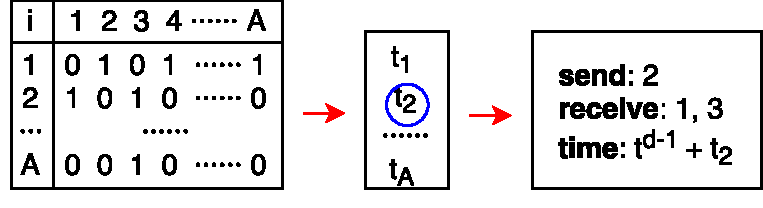
\includegraphics[width=0.57\textwidth]{figures/tie.pdf}
 \end{figure}	
\end{frame}

\begin{frame}{Inference - Pseudocode}
	\bni
	\item Bayesian Inference using Markov Chain Monte Carlo (MCMC)
  	\begin{center}
  		\scalebox{0.85}{	 
 	 \begin{minipage}{1\linewidth}\begin{algorithm}[H]
\SetAlgoLined
	 	\caption{MCMC}
	 	Set initial values $\mathcal{Z}^{(0)}, \mathcal{C}^{(0)}, $ and $(\mathcal{B}^{(0)}, \delta^{(0)})$\\
	 	\For{o=1 to O}{
	 				Sample the \textcolor{blue}{latent edge} $J^{(d)}_{ij}$ via Gibbs sampling\\\\
	 				Sample the \textcolor{blue}{topic assignments} $\mathcal{Z}$ via Gibbs sampling\\\\
	 			Sample the \textcolor{blue}{interaction pattern assignments} $\mathcal{C}$ via Gibbs sampling\\\\
	 		 				Sample the \textcolor{blue}{interaction pattern parameters} $\mathcal{B}$  via Metropolis-Hastings \\\\
	 			Sample the \textcolor{blue}{receiver size parameter} $\delta$ via Metropolis-Hastings
	 	}
	 \end{algorithm}
	\end{minipage}}
	 	\end{center}
	 		\ei
\end{frame}

\begin{frame}{Data: North Carolina Dare county email data}
 \bni \item $D = 1456$ emails between $A = 27$ county government managers, covering 2 month periods (October 1 - November 30) in 2012
 \begin{figure}
 	\includegraphics[width=0.55\textwidth]{figures/Dare.png}
 \end{figure}	
\vspace{0.4cm}
 \item Hurricane Sandy passed by NC: October 26 - October 30
 \ei
\end{frame}

\begin{frame}{Exploratory Data Analysis: Effect of Sandy}
	\begin{minipage}{0.85\linewidth}
	 	 \begin{figure}
	 	 	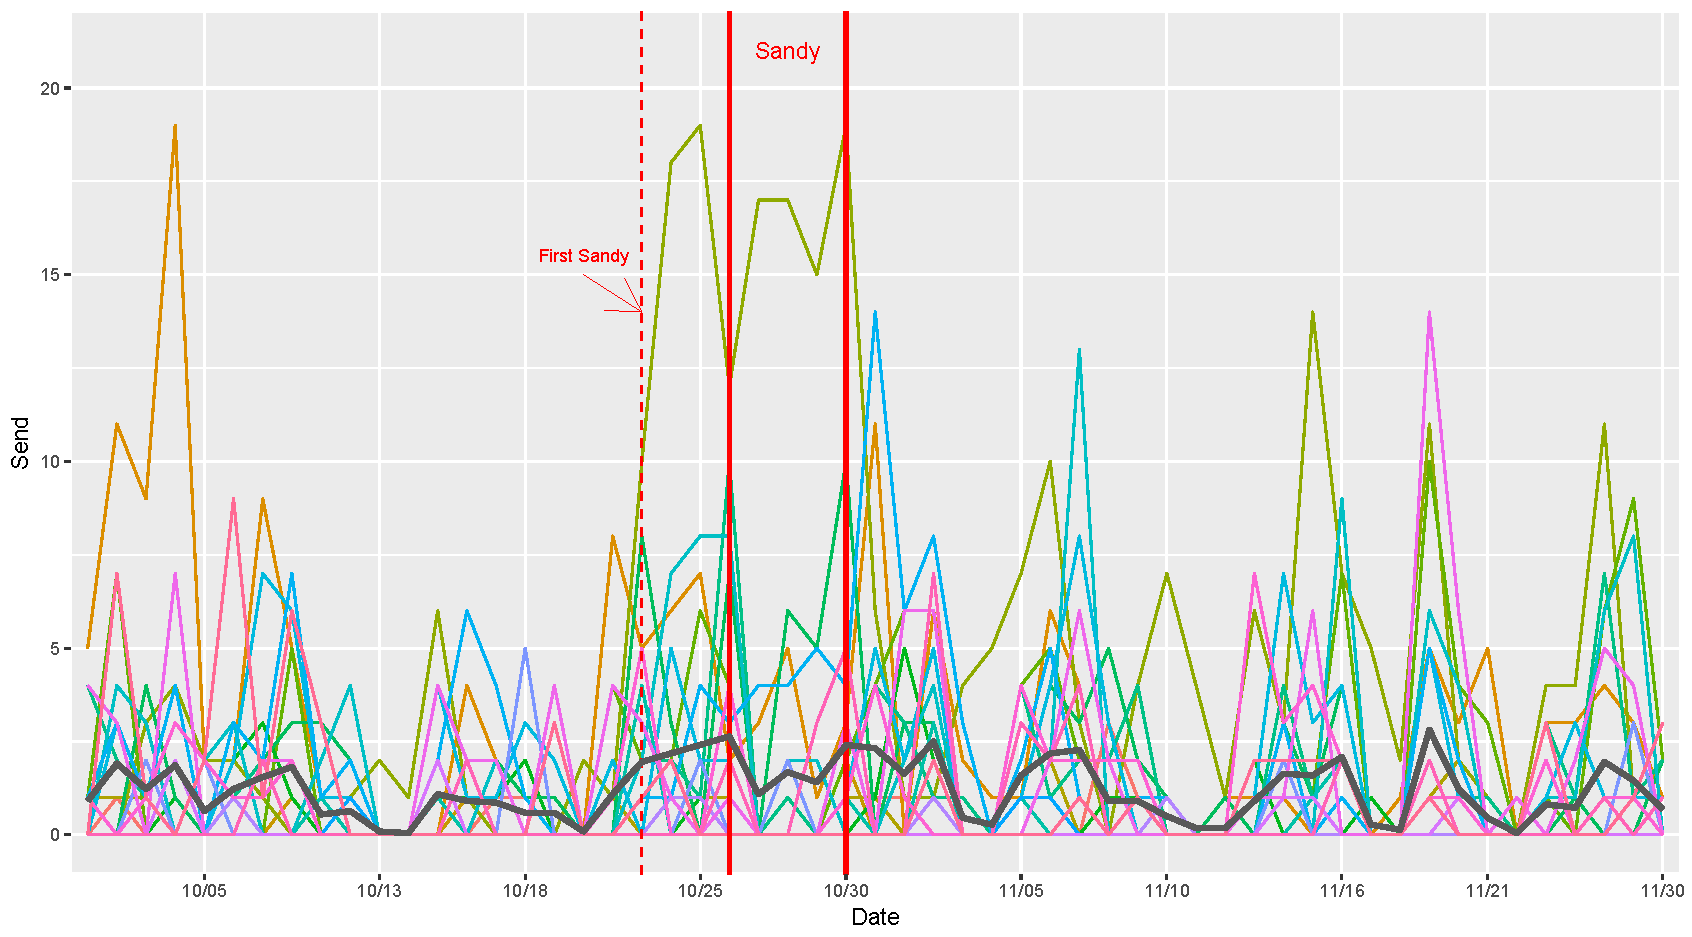
\includegraphics[width=0.5\textwidth]{figures/Sendplot.pdf}	 	
	 	 	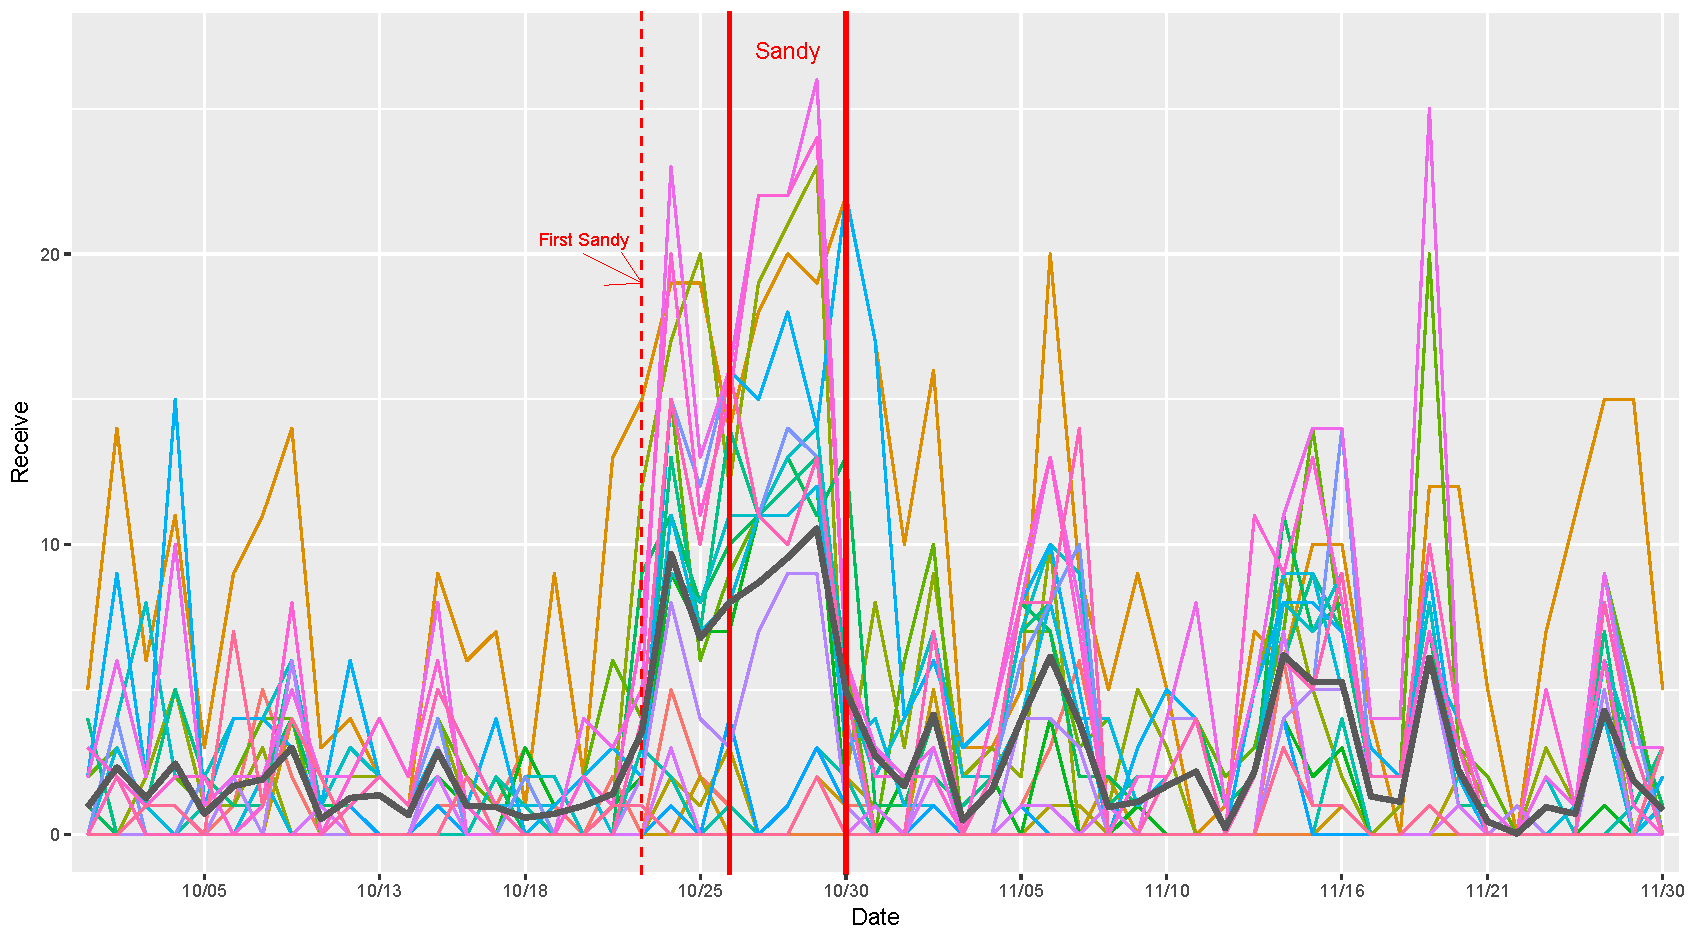
\includegraphics[width=0.5\textwidth]{figures/Receiveplot.pdf}
	 	 \end{figure}	
	 \begin{figure}
	 %	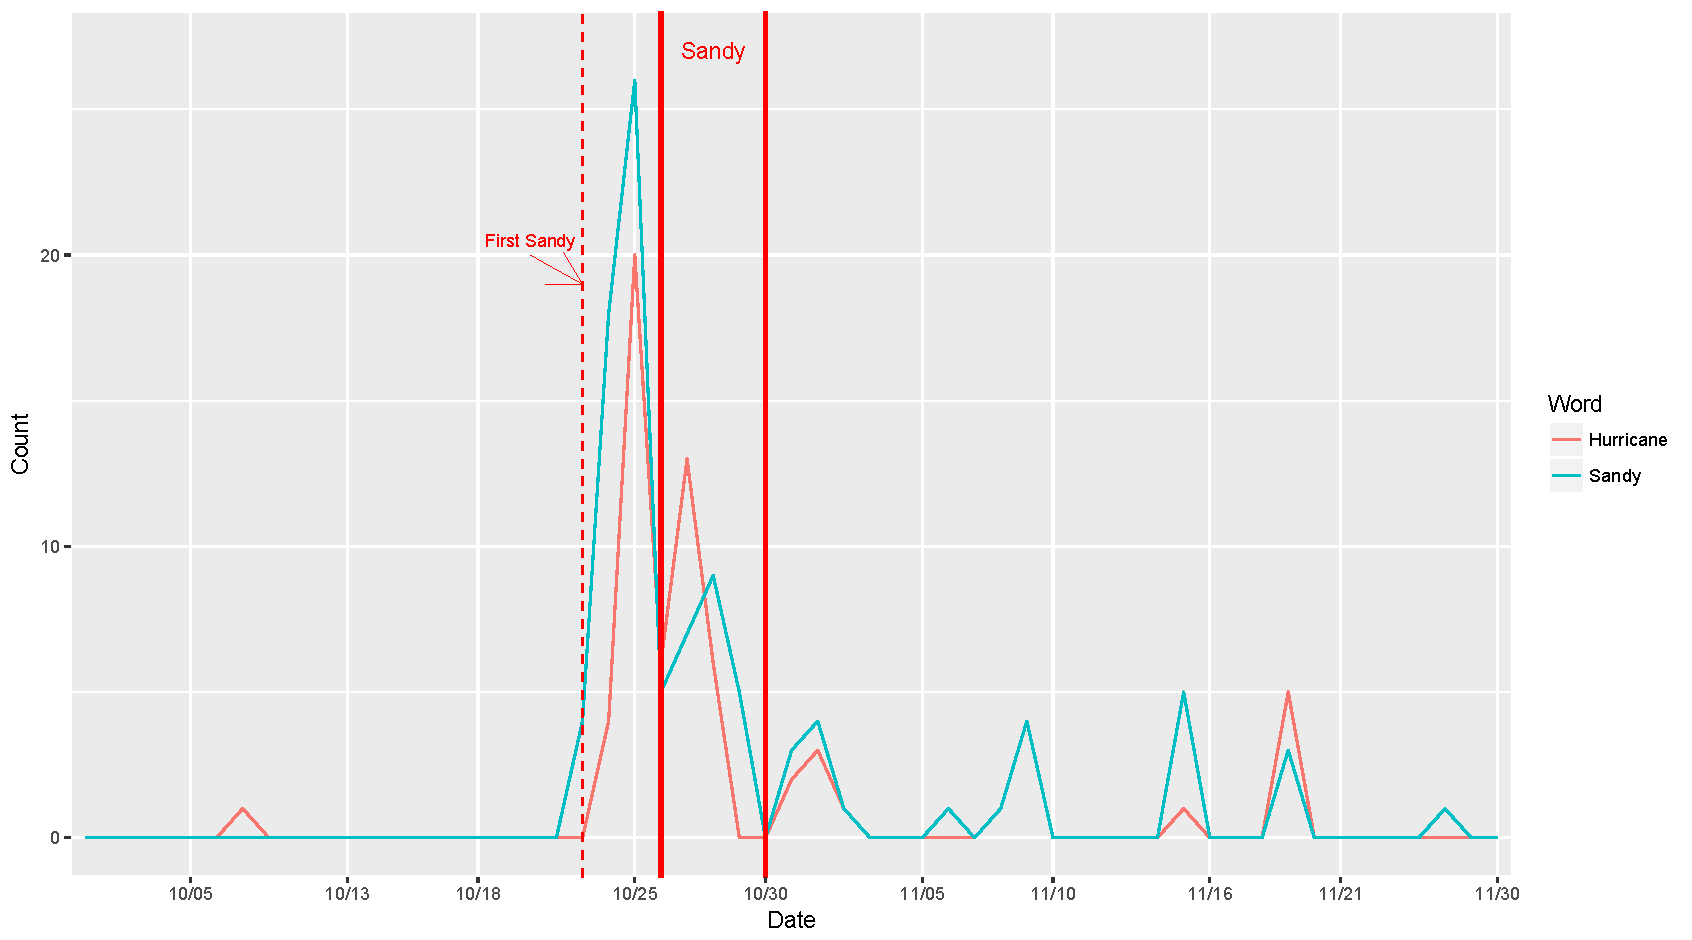
\includegraphics[width=0.5\textwidth]{Wordplot.pdf}	 
	 		 	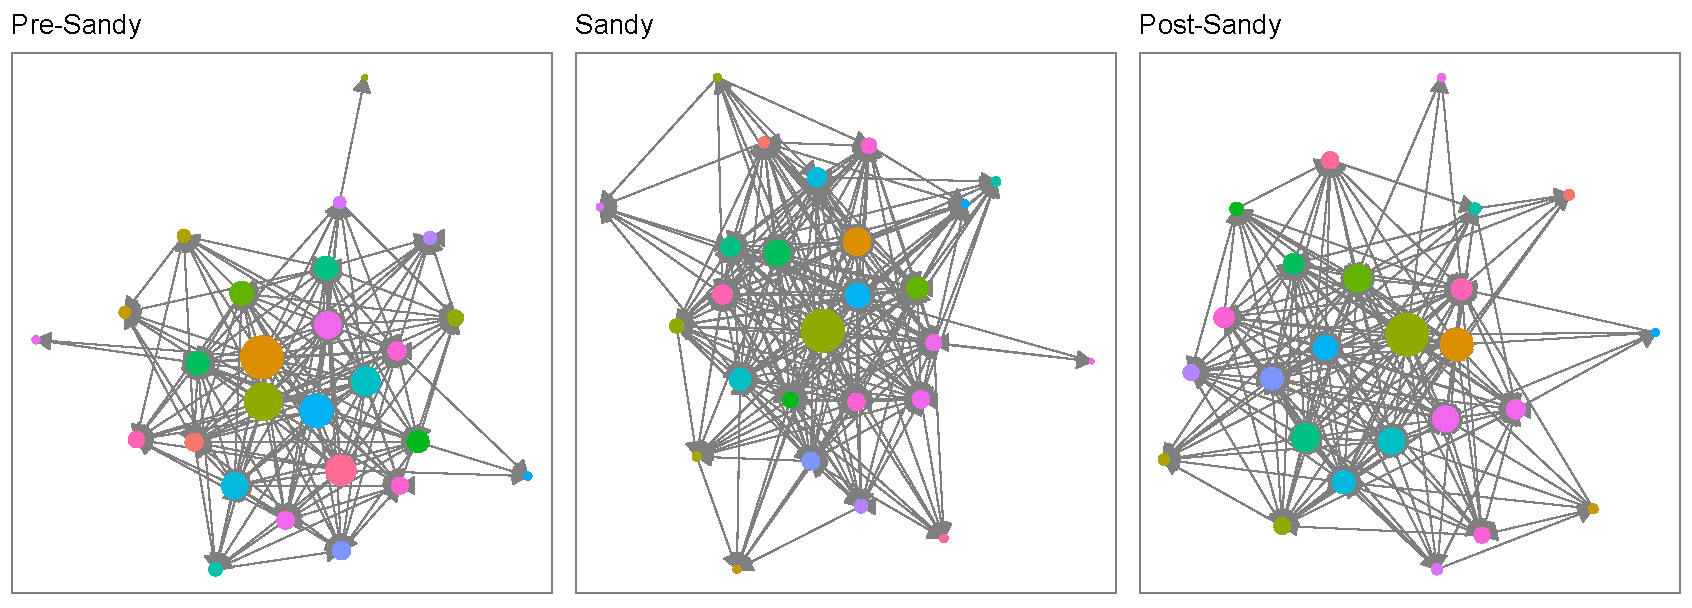
\includegraphics[width=1\textwidth]{figures/Networkplot.pdf}
	 		 		 \end{figure}	
\end{minipage}
\begin{minipage}{0.13\linewidth}
		 \begin{figure}
	 		 		 	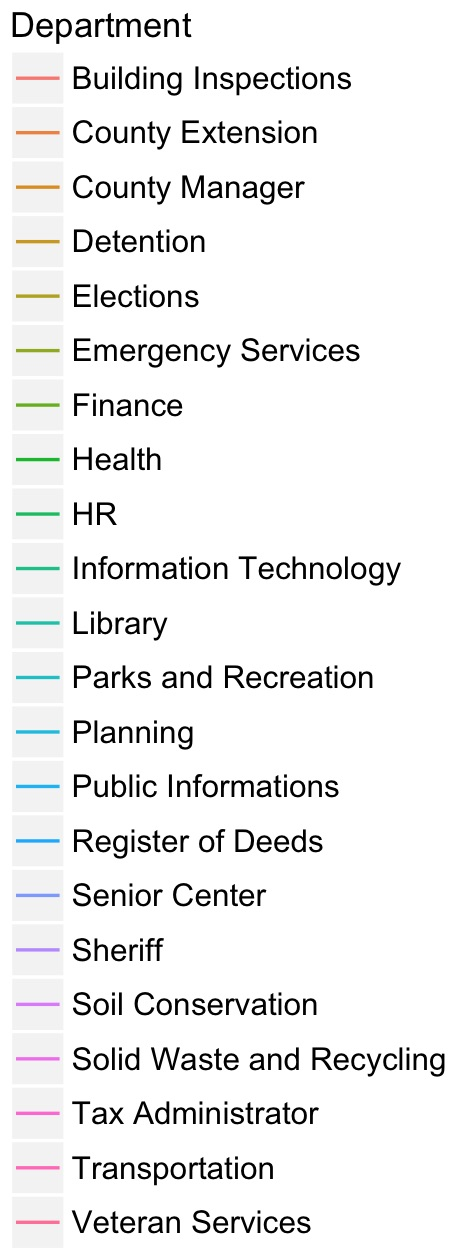
\includegraphics[width=1.25\textwidth]{figures/Dept2.jpg}
	 \end{figure}	
	\end{minipage}
\end{frame}
 \begin{frame}{IPTM Result: Contents}
 	\bni \item IPTM result with $C=2$, $K=20$ and $O= 20$\footnote{Preliminary results with small outer iterations. Model results subject to change.}:
 	\ei
 	\scriptsize
\centering	\begin{table}[ht]
	\centering
	\begin{tabular}{ |c||c|c|c||c|c|c|} 
		\hline
		\textbf{IP} & \textbf{1} &  \textbf{1} & \textbf{1}  &\textbf{2} &\textbf{2}  &\textbf{2}  \\ \hline\hline
			\textbf{Topic} & \textbf{2} &  \textbf{13} & \textbf{7}  &\textbf{10} &\textbf{9}  &\textbf{12}  \\ \hline\hline
			\textbf{Word}& winds & track & offices & sanitation & marshall & morning\\
			&flooding & offices & hurricane & billed & human & fema\\
			&policy & obx & sandy & long & collins & weather\\
			&mph & shore &  update & bill & phone & ems\\
			&moving & winds & force & question & resources & risks \\
			&outer & exam & reading & staff & phr & sure\\
			&banks & area &  contact & vehicles & drive & tomorrow\\
			&rain & change & updates & additional & box & opening\\
			&will & continues & amount & form & fax & address\\
			&duration & expect & northwest &  estimate & bridge &  elections\\
			&monday & curves & tuesday &  total & director & thought\\
			&ocean & side & expected & doors & monday & minutes \\
			&open & east & good & services & manteo & starting\\
			&heads & better &  well & tomorrow & summary & wrote\\
			&late & mile & night & haterras & october & operation\\
			
				\hline
	\end{tabular}
\end{table}
\normalsize
\end{frame}
\begin{frame}{IPTM Result: Dynamic Network Effects}
	\bni \item IPTM result with $C=2$, $K=20$ and $O= 20$\footnote{Preliminary results with small outer iterations. Model results subject to change.}:
	\ei
	\begin{figure}
		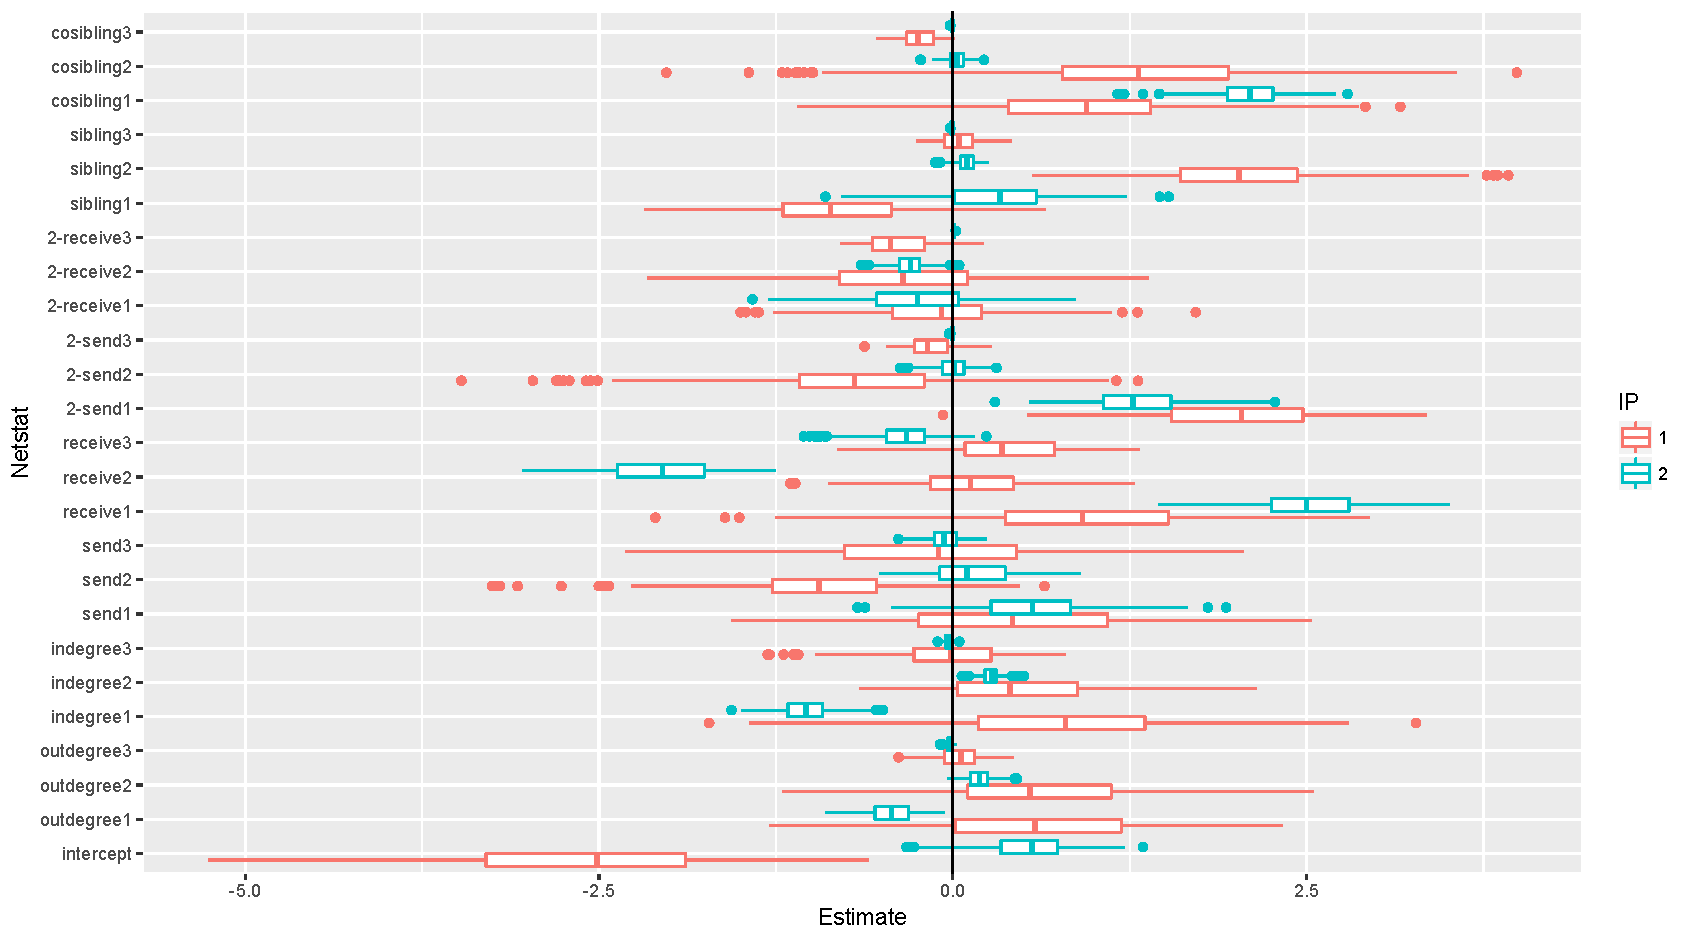
\includegraphics[width=1\textwidth]{figures/DareBplot.pdf}
	\end{figure}	
\end{frame}
\begin{frame}{Conclusion}
 \bni
 \item Joint modeling of ties (sender, receiver, time) and contents
 	\vspace{0.4cm}
 \item Allowance of multicast -- single sender and multiple receivers
 	\vspace{0.4cm}
 \item Possible application to various political science data
 \ei
\end{frame}
\end{document}